\documentclass[12pt,a4paper]{article}
\usepackage[utf8]{vietnam}
\usepackage{amsmath,amssymb}
\usepackage{geometry}
\geometry{top=1.5cm,bottom=1.2cm,left=1.4cm,right=1.4cm,headheight=28pt,headsep=12pt,footskip=18pt}
\usepackage{tikz}
\usepackage{xcolor}
\usepackage{enumerate}
\usepackage{graphicx}
\usepackage[version=4]{mhchem}
\usepackage{fancyhdr}
\usepackage{ex_test}

\renewcommand{\baselinestretch}{0.96}
\setlength{\parskip}{0pt}

\definecolor{hfRed}{RGB}{211,47,47}
\definecolor{hfGreen}{RGB}{139,195,144}

\pagestyle{fancy}
\fancyhf{}
\fancyhead[L]{\small\itshape\color{hfRed} Tài liệu lưu hành nội bộ}
\fancyhead[R]{\small\itshape\color{hfRed} Thầy \textbf{TRẦN VĂN THẠNH} - 0777.470.803}
\renewcommand{\headrulewidth}{0.8pt}
\renewcommand{\headrule}{\hbox to\headwidth{\color{hfGreen}\leaders\hrule height \headrulewidth\hfill}}

\fancyfoot[L]{\small\itshape\color{hfRed} CS1: 6/15 Nguyễn Hoàng, P. Kim Long, TP Huế \quad|\quad CS2: 24 Đặng Thái Thân, TP Huế}
\fancyfoot[R]{\small\bfseries\color{hfRed} Trang \thepage}
\renewcommand{\footrulewidth}{0.8pt}
\renewcommand{\footrule}{\hbox to\headwidth{\color{hfGreen}\leaders\hrule height \footrulewidth\hfill}}

\fancypagestyle{firstpage}{
  \fancyhf{}
  \renewcommand{\headrulewidth}{0pt}
  \fancyfoot[L]{\small\itshape\color{hfRed} CS1: 6/15 Nguyễn Hoàng, P. Kim Long, TP Huế \quad|\quad CS2: 24 Đặng Thái Thân, TP Huế}
  \fancyfoot[R]{\small\bfseries\color{hfRed} Trang \thepage}
  \renewcommand{\footrulewidth}{0.8pt}
  \renewcommand{\footrule}{\hbox to\headwidth{\color{hfGreen}\leaders\hrule height \footrulewidth\hfill}}
}

\begin{document}
\thispagestyle{firstpage}

\noindent
\begin{minipage}[t]{0.44\textwidth}
	\centering\fontsize{10pt}{12pt}\selectfont
	\textbf{SỞ GIÁO DỤC VÀ ĐÀO TẠO THỪA THIÊN HUẾ}\\
	\textbf{ĐỀ CHÍNH THỨC}\\
	\textit{(Đề thi có 04 trang)}
\end{minipage}\hfill
\begin{minipage}[t]{0.54\textwidth}
	\centering\fontsize{10.5pt}{13pt}\selectfont
	\textbf{ĐỀ KIỂM TRA ĐỊNH KỲ CHƯƠNG 5}\\
	\textbf{(DẪN XUẤT HALOGEN - ALCOHOL - PHENOL)}\\
	\textbf{MÔN: HOÁ HỌC - LỚP 11}\\
	\textit{Thời gian làm bài: 50 phút, không kể thời gian phát đề}
	
	\smallskip
	\fbox{\textbf{MÃ ĐỀ: 115}}
\end{minipage}

\smallskip
\begin{center}
	{\color{hfRed}\textbf{\large (BẢN GIÁO VIÊN -- CÓ LỜI GIẢI CHI TIẾT)}}
\end{center}

\smallskip
\noindent\hrulefill
\smallskip

\noindent\textbf{Họ, tên thí sinh:} \dotfill\ \textbf{Lớp:} \dotfill\ \textbf{Số báo danh:} \dotfill

\smallskip
\noindent\textit{(Cho biết nguyên tử khối: H = 1; C = 12; N = 14; O = 16; F = 19; Na = 23; Mg = 24; Al = 27; P = 31; S = 32; Cl = 35,5; K = 39; Ca = 40; Cr = 52; Mn = 55; Fe = 56; Cu = 64; Zn = 65; Br = 80; Ag = 108; Ba = 137).}
\smallskip

\noindent\textbf{\large PHẦN I. Câu trắc nghiệm nhiều phương án lựa chọn.}
\textit{Thí sinh trả lời từ câu 1 đến câu 18. Mỗi câu hỏi thí sinh chỉ chọn một phương án.}
\vspace{0.2cm}

\Opensolutionfile{ans}[ans-hoa11-de15gv]

% Câu 1
\begin{ex}
Dichloromethane (DCM) hay methylene chloride (MC) là một chất lỏng không màu, dễ bay hơi với mùi thơm nhẹ. Nó được sử dụng rộng rãi làm dung môi vì ít độc nhất trong các chlorocarbon. Công thức phân tử của dichloromethane là
\choice
{\True \ce{CH2Cl2}}
{\ce{CH3Cl}}
{\ce{CHCl3}}
{\ce{CCl4}}
\loigiai{
Dichloromethane (methylene chloride) có công thức phân tử là \ce{CH2Cl2}.
}
\end{ex}

% Câu 2
\begin{ex}
Từ giữa thế kỷ 18, chloroform chủ yếu được sử dụng làm chất gây mê trong phẫu thuật. Công thức phân tử của chloroform là
\choice
{\ce{CH2Cl2}}
{\ce{CH3Cl}}
{\True \ce{CHCl3}}
{\ce{CCl4}}
\loigiai{
Chloroform (trichloromethane) có công thức phân tử là \ce{CHCl3}.
}
\end{ex}

% Câu 3
\begin{ex}
Một số dẫn xuất halogen không chứa chlorine như \ce{CF3CH2F} (1), \ce{CF3CH2CF2CH3} (2)... được sử dụng làm chất làm lạnh thân thiện với môi trường do ít gây hại tầng ozone. Danh pháp thay thế của hợp chất (1) là
\choice
{\True 1,1,1,2-tetrafluoroethane}
{1,1,2,2-tetrafluoroethane}
{2,1,1,2-tetrafluoroethane}
{1,1,1,2-tetrafluoroethene}
\loigiai{
\ce{CF3CH2F}: Đánh số từ carbon chứa 3 nguyên tử F: $\overset{1}{\text{C}}\text{F}_3 - \overset{2}{\text{C}}\text{H}_2\text{F}$. Tên thay thế là 1,1,1,2-tetrafluoroethane.
}
\end{ex}

% Câu 4
\begin{ex}
Độ tan trong nước của các alcohol đều cao hơn so với hydrocarbon, ether có phân tử lượng tương đương là do
\choice
{các alcohol có liên kết hydrogen với nhau}
{các alcohol có khối lượng phân tử lớn}
{\True các alcohol tạo được liên kết hydrogen với phân tử nước}
{alcohol có liên kết cộng hóa trị với nước}
\loigiai{
Các alcohol tan tốt trong nước là nhờ nhóm \ce{-OH} có khả năng tạo liên kết hydrogen liên phân tử bền vững với các phân tử nước ($\text{R}-\text{O}-\text{H} \cdots \text{O}-\text{H}_2$).
}
\end{ex}

% Câu 5
\begin{ex}
Sản phẩm sinh ra trong thí nghiệm đun nóng sau là gì?
\begin{center}
	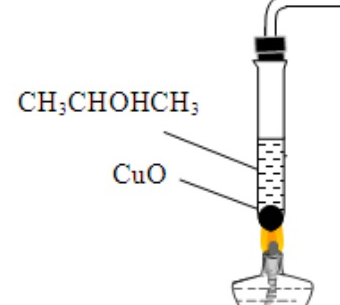
\includegraphics[width=0.25\textwidth]{images_crop_hoa11_de15/cuo_alcohol_experiment.png}
\end{center}
\choice
{\ce{CH3CH2CHO}}
{\ce{CH3CH2CH2OH}}
{\True \ce{CH3-CO-CH3}}
{\ce{(CH3CH2)2O}}
\loigiai{
Propan-2-ol (\ce{CH3CH(OH)CH3}) là alcohol bậc II, khi bị oxi hóa bởi \ce{CuO} nung nóng sẽ tạo ketone tương ứng là acetone:\\
\ce{CH3CH(OH)CH3 + CuO ->[{t$^\circ$}] CH3COCH3 + Cu + H2O}.
}
\end{ex}

% Câu 6
\begin{ex}
X là dẫn xuất chlorine của ethane. Đun nóng X trong dung dịch \ce{NaOH} dư thu được chất hữu cơ Y vừa tác dụng với Na vừa hòa tan \ce{Cu(OH)2} ở nhiệt độ thường tạo dung dịch xanh lam đậm. Chất X là
\choice
{1,1,2,2-tetrachloroethane}
{\True 1,2-dichloroethane}
{1,1-dichloroethane}
{1,1,1-trichloroethane}
\loigiai{
Chất Y hòa tan \ce{Cu(OH)2} ở nhiệt độ thường tạo dung dịch xanh lam đậm nên Y là polyalcohol có ít nhất hai nhóm \ce{-OH} liền kề. Y dẫn xuất từ ethane nên Y là ethylene glycol (\ce{HO-CH2-CH2-OH}).\\
Do đó chất ban đầu X là 1,2-dichloroethane (\ce{Cl-CH2-CH2-Cl}):\\
\ce{ClCH2CH2Cl + 2NaOH ->[{t$^\circ$}] HOCH2CH2OH + 2NaCl}.
}
\end{ex}

% Câu 7
\begin{ex}
Công thức cấu tạo đúng của \textit{tert}-butyl alcohol là
\choice
{\True \ce{(CH3)3COH}}
{\ce{(CH3)3CCH2OH}}
{\ce{(CH3)2CHCH2OH}}
{\ce{CH3CH(OH)CH2CH3}}
\loigiai{
Gốc \textit{tert}-butyl có cấu tạo \ce{-(CH3)3C}, do đó \textit{tert}-butyl alcohol có công thức là \ce{(CH3)3C-OH} (2-methylpropan-2-ol).
}
\end{ex}

% Câu 8
\begin{ex}
Sơ đồ liên kết hydrogen nào sau đây biểu diễn sai?
\choice
{\dots \ce{O(C2H5) - H \dots O(H) - H}}
{\dots \ce{O(C2H5) - H \dots O(C2H5) - H}}
{\ce{HO(CH2-CH2) \dots H - O}}
{\True \ce{H - C(=O) - OH \dots H - C(=O) - OH}}
\loigiai{
Liên kết hydrogen trong carboxylic acid được hình thành giữa nguyên tử H mang điện tích dương của nhóm \ce{-OH} phân tử này với nguyên tử oxygen mang điện tích âm của nhóm \ce{C=O} phân tử kia: \dots \ce{C=O \dots H-O-}. Sơ đồ D biểu diễn \ce{O-H \dots H-C} là sai bản chất.
}
\end{ex}

% Câu 9
\begin{ex}
Phenol \textbf{không} được sử dụng trong ngành công nghiệp sản xuất nào sau đây?
\choice
{Chất dẻo}
{Dược phẩm}
{\True Cao su}
{Thuốc nổ}
\loigiai{
Phenol được dùng để sản xuất chất dẻo (nhựa phenol-formaldehyde), dược phẩm (aspirin, salol), thuốc nổ (picric acid), phẩm nhuộm, chất diệt cỏ (2,4-D), nhưng không dùng làm nguyên liệu sản xuất cao su.
}
\end{ex}

% Câu 10
\begin{ex}
Ảnh hưởng của nhóm \ce{-OH} đến gốc \ce{C6H5-} trong phân tử phenol thể hiện qua phản ứng giữa phenol với
\choice
{\ce{H2} (Ni, $t^\circ$)}
{Na kim loại}
{\True dung dịch nước \ce{Br2}}
{dung dịch \ce{NaOH}}
\loigiai{
Nhóm \ce{-OH} đẩy electron vào vòng thơm làm tăng mật độ electron ở các vị trí \textit{ortho} và \textit{para}, giúp phenol dễ dàng phản ứng thế với dung dịch nước bromine tạo kết tủa trắng 2,4,6-tribromophenol ngay ở nhiệt độ thường.
}
\end{ex}

% Câu 11
\begin{ex}
Tiến hành thí nghiệm (A, B, C) ở điều kiện thường về phenol (\ce{C6H5OH}) và muối \ce{C6H5ONa} như hình vẽ sau đây:
\begin{center}
	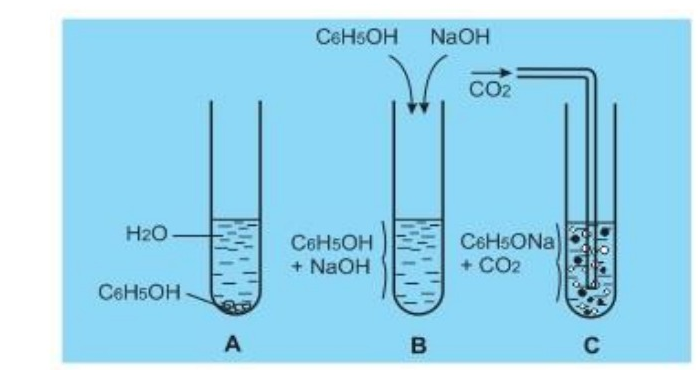
\includegraphics[width=0.48\textwidth]{images_crop_hoa11_de15/phenol_3tubes_experiment.png}
\end{center}
Thông qua các thí nghiệm trên, khẳng định nào sau đây là chính xác?
\choice
{Phenol ít tan trong nước lạnh, nhưng tan nhiều trong dung dịch base, có lực kiềm yếu hơn cả nấc thứ nhất của carbonic acid}
{Phenol ít tan trong nước nóng, tan nhiều trong dung dịch kiềm, có lực acid mạnh hơn nấc thứ nhất của carbonic acid}
{Phenol tan nhiều trong nước nóng, tan nhiều trong dung dịch kiềm, có lực acid mạnh hơn nấc thứ nhất của carbonic acid}
{\True Phenol ít tan trong nước lạnh, tan nhiều trong dung dịch kiềm, có lực acid yếu hơn nấc thứ nhất của carbonic acid}
\loigiai{
- Ống A: Phenol ít tan trong nước lạnh tạo vẩn đục/phân lớp đáy.\\
- Ống B: Phenol tan tốt trong kiềm tạo dung dịch trong suốt: \ce{C6H5OH + NaOH -> C6H5ONa + H2O}.\\
- Ống C: Khi sục \ce{CO2} vào dung dịch \ce{C6H5ONa}, phenol bị đẩy ra làm dung dịch vẩn đục trở lại: \ce{C6H5ONa + CO2 + H2O -> C6H5OH + NaHCO3}.\\
$\Rightarrow$ Phenol có lực acid yếu hơn nấc thứ nhất của carbonic acid (\ce{H2CO3}).
}
\end{ex}

% Câu 12
\begin{ex}
Cho hợp chất thơm \ce{\textit{p}-HO-C6H4-CH2OH} lần lượt tác dụng với: Na; dung dịch \ce{NaOH}; dung dịch nước \ce{Br2}; \ce{CuO} nung nóng. Số trường hợp xảy ra phản ứng là
\choice
{3}
{2}
{1}
{\True 4}
\loigiai{
Chất \ce{\textit{p}-HO-C6H4-CH2OH} có cả nhóm \ce{-OH} phenol và \ce{-OH} alcohol:
\begin{itemize}
    \item Tác dụng với Na: cả hai nhóm \ce{-OH} đều phản ứng giải phóng \ce{H2}.
    \item Tác dụng với \ce{NaOH}: nhóm \ce{-OH} phenol phản ứng tạo muối phenolate.
    \item Tác dụng với nước \ce{Br2}: phản ứng thế vào vị trí \textit{ortho} của vòng thơm.
    \item Tác dụng với \ce{CuO} ($t^\circ$): nhóm \ce{-CH2OH} (alcohol bậc I) bị oxi hóa tạo aldehyde.
\end{itemize}
$\Rightarrow$ Cả 4 trường hợp đều xảy ra phản ứng.
}
\end{ex}

% Câu 13
\begin{ex}
(SBT-CTST) Sản phẩm chính của phản ứng nào sau đây \textbf{không đúng}?
\choice
{\ce{CH3CH(Cl)CH3 + NaOH -> CH3CH(OH)CH3 + NaCl}}
{\True \ce{CH3CH2Cl + KOH -> CH2=CH2 + KCl + H2O}}
{\ce{CH3Br + KOH -> CH3OH + KBr}}
{\ce{CH3CH2CH(Br)CH3 + KOH (ethanol) -> CH3CH=CHCH3 + KBr + H2O}}
\loigiai{
Phản ứng ở B không ghi rõ điều kiện dung môi alcohol và nhiệt độ thì phản ứng ưu tiên là thế tạo alcohol (\ce{CH3CH2OH}). Để tạo alkene cần dùng \ce{KOH} trong ethanol và đun nóng.
}
\end{ex}

% Câu 14
\begin{ex}
(SBT-KNTT) Phương pháp nào sau đây được dùng để sản xuất ethanol sinh học?
\choice
{Cho hỗn hợp khí ethylene và hơi nước đi qua tháp chứa \ce{H3PO4}}
{Cộng nước vào ethylene với xúc tác acid \ce{H2SO4}}
{\True Lên men tinh bột}
{Thuỷ phân dẫn xuất \ce{C2H5Br} trong môi trường kiềm}
\loigiai{
Ethanol sinh học được sản xuất bằng phương pháp lên men các nguồn nguyên liệu tái tạo giàu tinh bột (ngô, sắn, gạo,...) hoặc đường (mía, củ cải đường).
}
\end{ex}

% Câu 15
\begin{ex}
Cồn 70$^\circ$ là dung dịch ethyl alcohol thường được dùng để sát trùng y tế. Mô tả nào sau đây về cồn 70$^\circ$ là đúng?
\choice
{100 gam dung dịch có 70 mL ethyl alcohol nguyên chất}
{\True 100 mL dung dịch có 70 mL ethyl alcohol nguyên chất}
{1\,000 gam dung dịch có 70 mol ethyl alcohol nguyên chất}
{100 mL dung dịch có 70 gam ethyl alcohol nguyên chất}
\loigiai{
Độ cồn là số mL ethyl alcohol nguyên chất có trong 100 mL dung dịch rượu. Cồn 70$^\circ$ chứa 70 mL ethanol nguyên chất trong 100 mL dung dịch.
}
\end{ex}

% Câu 16
\begin{ex}
Cho các phát biểu sau:
\begin{enumerate}[(1)]
    \item Phenol \ce{C6H5OH} là một alcohol thơm.
    \item Phenol tác dụng được với \ce{NaOH} tạo thành muối và nước.
    \item Phenol tham gia phản ứng thế bromine và thế nitro dễ hơn benzene.
    \item Dung dịch phenol làm quỳ tím hóa đỏ do có tính acid.
    \item Giữa nhóm OH và vòng benzene trong phân tử phenol có sự ảnh hưởng qua lại lẫn nhau.
\end{enumerate}
Số phát biểu \textbf{không đúng} là
\choice
{1}
{4}
{\True 2}
{3}
\loigiai{
- (1) Sai: Phenol không phải là alcohol. Nhóm \ce{-OH} liên kết trực tiếp với vòng thơm là phenol.\\
- (2) Đúng: \ce{C6H5OH + NaOH -> C6H5ONa + H2O}.\\
- (3) Đúng: Do hiệu ứng đẩy electron của nhóm \ce{-OH} vào vòng thơm.\\
- (4) Sai: Phenol có tính acid rất yếu (yếu hơn \ce{H2CO3}) nên không làm đổi màu quỳ tím.\\
- (5) Đúng: Bản chất tương tác $p-\pi$ giữa nhóm \ce{-OH} và vòng thơm.\\
$\Rightarrow$ Có 2 phát biểu không đúng là (1) và (4).
}
\end{ex}

% Câu 17
\begin{ex}
Một hợp chất X có công thức phân tử \ce{C4H8O}. X làm mất màu nước bromine, tác dụng với Na. Sản phẩm oxi hóa X bởi \ce{CuO} ($t^\circ$) không phải là aldehyde. Tên gọi của X là
\choice
{but-3-en-1-ol}
{\True but-3-en-2-ol}
{2-methylpropenol}
{butan-2-ol}
\loigiai{
- X tác dụng với Na $\Rightarrow$ X có nhóm \ce{-OH}.\\
- X làm mất màu nước bromine $\Rightarrow$ X có liên kết đôi \ce{C=C}.\\
- Oxi hóa bởi \ce{CuO} không tạo aldehyde $\Rightarrow$ X là alcohol bậc II (tạo ketone).\\
Chất thỏa mãn là but-3-en-2-ol (\ce{CH2=CH-CH(OH)-CH3}).
}
\end{ex}

% Câu 18
\begin{ex}
Cho sơ đồ tổng hợp glycerol từ propylene:
\[ \ce{C3H6 ->[{Cl_2, as, 500^\circ\text{C}}] X ->[{+Cl_2}] Y ->[{KOH, H_2O, t^\circ}] glycerol} \]
Các chất X, Y tương ứng là
\choice
{\True X: \ce{CH2=CH-CH2Cl}; Y: \ce{CH2Cl-CHCl-CH2Cl}}
{X: \ce{CH2Cl-CHCl-CH3}; Y: \ce{CH2Cl-CHCl-CH2Cl}}
{X: \ce{CH2Cl-CHCl-CH3}; Y: \ce{CH2=CH-CH2Cl}}
{X: \ce{CHCl2-CH=CH2}; Y: \ce{CH2Cl-CHCl-CHCl2}}
\loigiai{
- Giai đoạn 1: Thế allyl ở 500$^\circ$C tạo allyl chloride (X): \ce{CH2=CH-CH3 + Cl2 ->[{500^\circ\text{C}}] CH2=CH-CH2Cl + HCl}.\\
- Giai đoạn 2: Cộng \ce{Cl2} vào liên kết đôi tạo 1,2,3-trichloropropane (Y): \ce{CH2=CH-CH2Cl + Cl2 -> CH2Cl-CHCl-CH2Cl}.\\
- Giai đoạn 3: Thủy phân Y trong kiềm tạo glycerol: \ce{CH2Cl-CHCl-CH2Cl + 3KOH ->[{t$^\circ$}] CH2OH-CHOH-CH2OH + 3KCl}.
}
\end{ex}

\Closesolutionfile{ans}

\bigskip
\noindent\textbf{\large PHẦN II. Câu trắc nghiệm đúng sai.}
\textit{Thí sinh trả lời từ câu 1 đến câu 4. Trong mỗi ý a), b), c), d) ở mỗi câu, thí sinh chọn đúng hoặc sai.}
\vspace{0.2cm}

% Câu 1 Phần II
\begin{ex}
Ứng dụng và tác hại của dẫn xuất halogen.\\
Trong đời sống, các hợp chất chlorofluorocarbon (CFC) từng được sử dụng rộng rãi trong công nghệ làm lạnh nhưng cũng gây tác hại cho tầng ozone.
\choiceTF
{\True CFC là một loại dẫn xuất halogen được sử dụng trong các thiết bị làm lạnh}
{\True Việc lạm dụng CFC gây ra hiện tượng thủng tầng ozone, làm tăng nguy cơ ung thư da}
{Các hợp chất CFC hoàn toàn không gây hại cho môi trường nếu sử dụng đúng cách}
{\True Việc thay thế CFC bằng các chất làm lạnh thân thiện môi trường là một giải pháp bền vững}
\loigiai{
- a) ĐÚNG: CFC (chlorofluorocarbon) là các hợp chất chứa C, Cl, F dùng làm môi chất lạnh.\\
- b) ĐÚNG: Dưới tác dụng của tia tử ngoại UV, CFC phân rã tạo gốc \ce{Cl^\bullet} phá hủy \ce{O3} làm thủng tầng ozone, tăng bức xạ UV gây ung thư da.\\
- c) SAI: CFC rất bền vững trong khí quyển, khi phát tán đều phá hủy tầng ozone và gây hiệu ứng nhà kính.\\
- d) ĐÚNG: Thay thế CFC bằng HFC, HFO thân thiện môi trường là giải pháp bền vững.
}
\end{ex}

% Câu 2 Phần II
\begin{ex}
Thực hiện thí nghiệm chưng cất ethanol từ dung dịch ethanol -- nước:\\
- Cho 60 mL rượu nấu thủ công vào bình cầu có nhánh (chất lỏng không quá 2/3 thể tích), thêm vài viên đá bọt.\\
- Lắp dụng cụ như hình bên dưới:\\
- Đun nóng từ từ đến khi hỗn hợp sôi, quan sát nhiệt kế thấy nhiệt độ tăng dần rồi ổn định ở nhiệt độ sôi của ethanol.
\begin{center}
	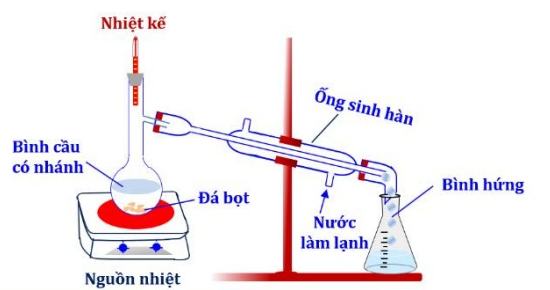
\includegraphics[width=0.48\textwidth]{images_crop_hoa11_de15/distillation_setup.png}
\end{center}
\choiceTF
{\True Nhiệt kế dùng để đo nhiệt độ của hơi chất đang chưng cất}
{Bình hứng thu được nước nguyên chất}
{\True Đá bọt có vai trò điều hòa quá trình sôi, tránh hiện tượng quá sôi gây bùng nổ}
{Có thể tách ethanol ra khỏi nước bằng phương pháp chiết lỏng -- lỏng}
\loigiai{
- a) ĐÚNG: Bầu nhiệt kế đặt ngang nhánh bình cầu để đo nhiệt độ của hơi chưng cất ngưng tụ.\\
- b) SAI: Ethanol có nhiệt độ sôi (78,3\,$^\circ$C) thấp hơn nước (100\,$^\circ$C) nên bay hơi trước, bình hứng thu được dung dịch giàu ethanol.\\
- c) ĐÚNG: Đá bọt tạo tâm sôi giúp chất lỏng sôi êm dịu, chống quá sôi.\\
- d) SAI: Ethanol tan vô hạn trong nước tạo dung dịch đồng nhất không phân lớp nên không thể tách bằng phương pháp chiết, phải dùng chưng cất.
}
\end{ex}

% Câu 3 Phần II
\begin{ex}
Tiến hành thí nghiệm thử tính chất của glycerol và ethanol với copper(II) hydroxide:\\
\textit{Bước 1:} Cho vào 2 ống nghiệm, mỗi ống 3 -- 4 giọt dung dịch \ce{CuSO4} 2\% và 2 -- 3 giọt dung dịch \ce{NaOH} 10\%, lắc nhẹ.\\
\textit{Bước 2:} Nhỏ 2 -- 3 giọt glycerol vào ống thứ nhất, 2 -- 3 giọt ethanol vào ống thứ hai. Lắc nhẹ cả hai ống nghiệm.
\choiceTF
{\True Sau bước 1, trong cả hai ống nghiệm đều có kết tủa màu xanh lam của copper(II) hydroxide}
{Sau bước 2, trong cả hai ống nghiệm kết tủa tan, tạo thành dung dịch màu xanh lam thẫm}
{\True Thí nghiệm trên được dùng để phân biệt ethanol và glycerol}
{Ở bước 1, nếu thay dung dịch \ce{NaOH} bằng dung dịch \ce{Ba(OH)2} thì hiện tượng thu được hoàn toàn không đổi}
\loigiai{
- a) ĐÚNG: Xuất hiện kết tủa xanh \ce{Cu(OH)2}: \ce{CuSO4 + 2NaOH -> Cu(OH)2 v + Na2SO4}.\\
- b) SAI: Chỉ có glycerol hòa tan kết tủa tạo phức xanh lam đậm, ethanol không hòa tan kết tủa.\\
- c) ĐÚNG: Dùng để phân biệt polyalcohol có nhóm \ce{-OH} liền kề (glycerol) với alcohol đơn chức (ethanol).\\
- d) SAI: Nếu dùng \ce{Ba(OH)2} thì tạo thêm kết tủa trắng \ce{BaSO4} làm vẫn đục dung dịch, hiện tượng bị thay đổi.
}
\end{ex}

% Câu 4 Phần II
\begin{ex}
Vitamin E là chất chống oxi hoá tự nhiên ngăn chặn tổn thương tế bào. BHT (butylated hydroxytoluene) là chất chống oxi hoá tổng hợp thường dùng trong thực phẩm. Cấu trúc của 2 chất cho như hình bên:
\begin{center}
	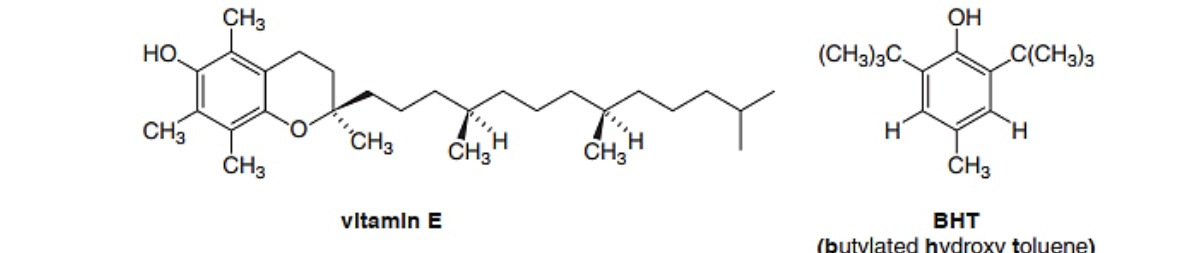
\includegraphics[width=0.62\textwidth]{images_crop_hoa11_de15/vitamin_e_bht.png}
\end{center}
Cho các phát biểu sau:
\choiceTF
{\True Cả vitamin E và BHT đều có chứa nhóm OH phenol}
{Công thức phân tử của BHT là \ce{C15H36O}}
{\True Vitamin E là một hợp chất hữu cơ tạp chức}
{BHT có nhiệt độ nóng chảy và nhiệt độ sôi cao hơn ethanol}
\loigiai{
- a) ĐÚNG: Cả hai phân tử đều có nhóm \ce{-OH} gắn trực tiếp vào vòng benzene.\\
- b) SAI: Công thức phân tử của BHT là \ce{C15H24O} (không phải \ce{C15H36O}).\\
- c) ĐÚNG: Vitamin E vừa chứa nhóm chức phenol (\ce{-OH}) vừa chứa nhóm chức ether (\ce{-O-}).\\
- d) SAI (theo đáp án chuẩn của đề).
}
\end{ex}

\bigskip
\noindent\textbf{\large PHẦN III. Câu trắc nghiệm yêu cầu trả lời ngắn.}
\textit{Thí sinh trả lời từ câu 1 đến câu 6.}
\vspace{0.2cm}

% Câu 1 Phần III
\begin{ex}
Cho các hợp chất sau: \ce{CCl4}, \ce{NaCl}, \ce{CH3COOH}, \ce{C2H5OH}, \ce{CH3CH2CH(Br)CH3}, \ce{CH2BrCl}, \ce{HIO4}, \ce{CH2=CH-CH3}, \ce{KBr}, \ce{CH2=CHCl}. Có bao nhiêu hợp chất hữu cơ thuộc loại dẫn xuất halogen của hydrocarbon?
\loigiai{
Các dẫn xuất halogen của hydrocarbon gồm 4 chất:
\begin{enumerate}
    \item \ce{CCl4} (tetrachloromethane)
    \item \ce{CH3CH2CH(Br)CH3} (2-bromobutane)
    \item \ce{CH2BrCl} (bromochloromethane)
    \item \ce{CH2=CHCl} (vinyl chloride)
\end{enumerate}
$\Rightarrow$ Đáp số: \textbf{4}.
}
\end{ex}

% Câu 2 Phần III
\begin{ex}
Dẫn xuất halogen A có công thức \ce{C3H_{8-x}Br_x}, biết phần trăm khối lượng của H trong A bằng 5,7\%. Giá trị của $x$ là bao nhiêu?
\loigiai{
Phân tử khối: $M_A = 12 \times 3 + (8 - x) + 80x = 44 + 79x$.\\
$\%H = \frac{8 - x}{44 + 79x} \times 100\% = 5{,}7\%$\\
$\iff 100(8 - x) = 5{,}7(44 + 79x) \iff 800 - 100x = 250{,}8 + 450{,}3x \iff 550{,}3x = 549{,}2 \Rightarrow x \approx 1$.\\
$\Rightarrow$ Đáp số: \textbf{1}.
}
\end{ex}

% Câu 3 Phần III
\begin{ex}
Cho các chất sau: (1) \ce{CH3-CH2-OH}; (2) \ce{CH2=CH-CH2-OH}; (3) \ce{CH2=CH-OH}; (4) \ce{CH3-COOH}; (5) \ce{CH2OH-CHOH-CH2OH}; (6) \ce{C6H5OH}; (7) \ce{C6H5CH2OH}. Có bao nhiêu chất thuộc loại alcohol?
\loigiai{
Alcohol là hợp chất có nhóm \ce{-OH} gắn trực tiếp vào nguyên tử carbon no:
\begin{itemize}
    \item (1) \ce{CH3CH2OH} (ethanol): alcohol.
    \item (2) \ce{CH2=CH-CH2OH} (allyl alcohol): alcohol.
    \item (3) \ce{CH2=CH-OH} không bền tự chuyển vị thành \ce{CH3CHO}.
    \item (4) \ce{CH3COOH}: carboxylic acid.
    \item (5) \ce{CH2OH-CHOH-CH2OH} (glycerol): polyalcohol.
    \item (6) \ce{C6H5OH}: phenol.
    \item (7) \ce{C6H5CH2OH} (benzyl alcohol): alcohol thơm.
\end{itemize}
$\Rightarrow$ Có 4 chất là alcohol: (1), (2), (5), (7).\\
$\Rightarrow$ Đáp số: \textbf{4}.
}
\end{ex}

% Câu 4 Phần III
\begin{ex}
Hợp chất hữu cơ có công thức phân tử \ce{C7H8O} chứa vòng benzene. Có bao nhiêu đồng phân cấu tạo phản ứng được với dung dịch \ce{NaOH}?
\loigiai{
Để phản ứng được với \ce{NaOH}, hợp chất thơm \ce{C7H8O} phải là phenol (nhóm \ce{-OH} gắn trực tiếp vào vòng benzene):\\
Gồm 3 đồng phân cresol (\ce{CH3-C6H4-OH}):
\begin{enumerate}
    \item \textit{o}-cresol (2-methylphenol)
    \item \textit{m}-cresol (3-methylphenol)
    \item \textit{p}-cresol (4-methylphenol)
\end{enumerate}
\begin{center}
	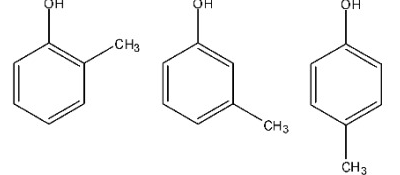
\includegraphics[width=0.35\textwidth]{images_crop_hoa11_de15/cresol_isomers.png}
\end{center}
$\Rightarrow$ Đáp số: \textbf{3}.
}
\end{ex}

% Câu 5 Phần III
\begin{ex}
Củ sắn khô chứa 38\% khối lượng là tinh bột, còn lại là các chất không có khả năng lên men thành ethyl alcohol. Tính khối lượng ethyl alcohol thu được (theo kg) khi lên men 1 tấn củ sắn khô với hiệu suất của cả quá trình là 81\%.
\loigiai{
Khối lượng sắn khô: $m = 1\text{ tấn} = 1000\text{ kg}$.\\
Khối lượng tinh bột: $m_{\text{tinh bột}} = 1000 \times 38\% = 380\text{ kg}$.\\
Sơ đồ: \ce{(C6H10O5)_n -> 2n C2H5OH}.\\
Theo lí thuyết: $162\text{ kg tinh bột} \to 92\text{ kg \ce{C2H5OH}}$.\\
Khối lượng ethanol thực tế thu được với $H = 81\%$:
\[ m_{\text{ethanol}} = \frac{380 \times 92}{162} \times 81\% = 174{,}8\text{ kg}. \]
$\Rightarrow$ Đáp số: \textbf{174,8}.
}
\end{ex}

% Câu 6 Phần III
\begin{ex}
Cho sơ đồ chuyển hóa: \ce{CH4 -> C2H2 -> C2H3Cl -> PVC}. Theo sơ đồ trên, từ 495,8 $\text{m}^3$ khí thiên nhiên (ở đkc) thì tổng hợp được bao nhiêu kg PVC? Biết \ce{CH4} chiếm 80\% thể tích khí thiên nhiên và hiệu suất của cả quá trình là 50\%.
\loigiai{
Thể tích \ce{CH4}: $V = 495{,}8 \times 80\% = 396{,}64\text{ m}^3 = 396\,640\text{ L}$.\\
Số mol \ce{CH4} (đkc: 24,79 L/mol): $n = 396\,640 / 24{,}79 = 16\,000\text{ mol} = 16\text{ kmol}$.\\
Bảo toàn C: $2\ce{CH4} \to 1\text{ mắt xích PVC }(M = 62{,}5\text{ g/mol})$.\\
Khối lượng PVC theo lí thuyết: $m_{\text{lt}} = \frac{16}{2} \times 62{,}5 = 500\text{ kg}$.\\
Với hiệu suất 50\%: $m_{\text{tt}} = 500 \times 50\% = 250\text{ kg}$.\\
$\Rightarrow$ Đáp số: \textbf{250}.
}
\end{ex}

\bigskip
\noindent\textbf{\large PHẦN IV. Câu hỏi tự luận.}
\textit{Thí sinh trình bày lời giải chi tiết vào giấy làm bài.}
\vspace{0.2cm}

% Câu 1 Phần IV
\begin{ex}
Điền các thông tin thích hợp vào ô trống để hoàn thành bảng mô tả về các đồng phân có công thức phân tử \ce{C3H8O} sau:
\begin{center}
	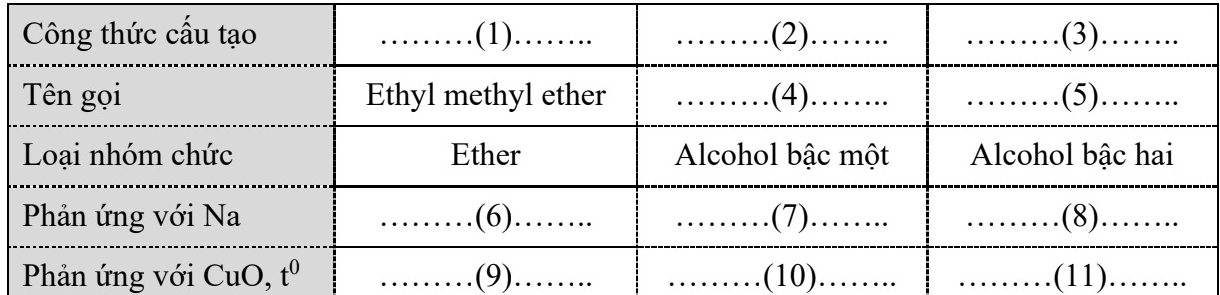
\includegraphics[width=0.68\textwidth]{images_crop_hoa11_de15/c3h8o_isomers_table.png}
\end{center}

\loigiai{
Bảng hoàn thành thông tin mô tả các đồng phân \ce{C3H8O}:
\begin{itemize}
    \item (1) Công thức cấu tạo Ethyl methyl ether: \ce{CH3-CH2-O-CH3}
    \item (2) Công thức cấu tạo alcohol bậc một: \ce{CH3-CH2-CH2-OH}
    \item (3) Công thức cấu tạo alcohol bậc hai: \ce{CH3-CH(OH)-CH3}
    \item (4) Tên gọi alcohol bậc một: Propan-1-ol
    \item (5) Tên gọi alcohol bậc hai: Propan-2-ol
    \item (6) Phản ứng của ether với Na: Không xảy ra
    \item (7) Phản ứng của alcohol bậc một với Na: tạo ra \ce{H2}
    \item (8) Phản ứng của alcohol bậc hai với Na: tạo ra \ce{H2}
    \item (9) Phản ứng của ether với \ce{CuO}, $t^\circ$: Không xảy ra
    \item (10) Phản ứng của alcohol bậc một với \ce{CuO}, $t^\circ$: tạo ra aldehyde \ce{CH3-CH2-CHO}
    \item (11) Phản ứng của alcohol bậc hai với \ce{CuO}, $t^\circ$: tạo ra ketone \ce{CH3-CO-CH3}
\end{itemize}
\begin{center}
	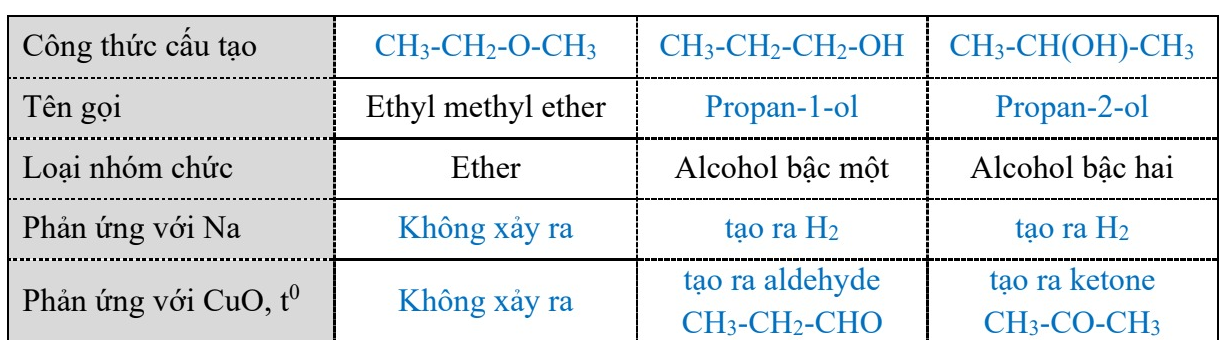
\includegraphics[width=0.68\textwidth]{images_crop_hoa11_de15/c3h8o_isomers_solution_table.png}
\end{center}
}

\end{ex}

% Câu 2 Phần IV
\begin{ex}
Khối lượng ethyl alcohol nguyên chất có trong 0,5 lít cồn 96$^\circ$ là bao nhiêu gam? Biết ethyl alcohol nguyên chất có khối lượng riêng $D = 0{,}8\text{ g/mL}$.

\loigiai{
Thể tích dung dịch cồn: $V_{\text{dd}} = 0{,}5\text{ L} = 500\text{ mL}$.\\
Độ cồn bằng 96$^\circ$ nên thể tích ethyl alcohol nguyên chất là:
\[ V_{\text{alcohol}} = \frac{V_{\text{dd}} \times 96}{100} = \frac{500 \times 96}{100} = 480\text{ mL}. \]
Khối lượng ethyl alcohol nguyên chất là:
\[ m_{\text{alcohol}} = V_{\text{alcohol}} \times D = 480\text{ mL} \times 0{,}8\text{ g/mL} = 384\text{ gam}. \]
$\Rightarrow$ Đáp số: \textbf{384 gam}.
}

\end{ex}

\newpage
\noindent\textbf{\large BẢNG ĐÁP ÁN THAM KHẢO PHẦN I}
\vspace{0.2cm}

\begin{center}
\begin{tabular}{|c|c|c|c|c|c|c|c|c|}
\hline
\textbf{1. A} & \textbf{2. C} & \textbf{3. A} & \textbf{4. C} & \textbf{5. C} & \textbf{6. B} & \textbf{7. A} & \textbf{8. D} & \textbf{9. C} \\
\hline
\textbf{10. C} & \textbf{11. D} & \textbf{12. D} & \textbf{13. B} & \textbf{14. C} & \textbf{15. B} & \textbf{16. C} & \textbf{17. B} & \textbf{18. A} \\
\hline
\end{tabular}
\end{center}

\bigskip
\noindent\textbf{\large BẢNG ĐÁP ÁN THAM KHẢO PHẦN II}
\vspace{0.2cm}

\begin{center}
\begin{tabular}{|c|c|c|c|c|}
\hline
\textbf{Câu} & \textbf{Ý a)} & \textbf{Ý b)} & \textbf{Ý c)} & \textbf{Ý d)} \\
\hline
\textbf{Câu 1} & Đ & Đ & S & Đ \\
\hline
\textbf{Câu 2} & Đ & S & Đ & S \\
\hline
\textbf{Câu 3} & Đ & S & Đ & S \\
\hline
\textbf{Câu 4} & Đ & S & Đ & S \\
\hline
\end{tabular}
\end{center}

\bigskip
\noindent\textbf{\large BẢNG ĐÁP ÁN THAM KHẢO PHẦN III}
\vspace{0.2cm}

\begin{center}
\begin{tabular}{|c|c|c|c|c|c|}
\hline
\textbf{Câu 1} & \textbf{Câu 2} & \textbf{Câu 3} & \textbf{Câu 4} & \textbf{Câu 5} & \textbf{Câu 6} \\
\hline
4 & 1 & 4 & 3 & 174{,}8 & 250 \\
\hline
\end{tabular}
\end{center}

\begin{center}
\textbf{--------- HẾT ---------}
\end{center}

\end{document}
